% Paper 2 · Figure 1: v0.8 pipeline diagram (TikZ)
% Render with: pdflatex pipeline_v08.tex
% Or include in main paper as: % Paper 2 · Figure 1: v0.8 pipeline diagram (TikZ)
% Render with: pdflatex pipeline_v08.tex
% Or include in main paper as: % Paper 2 · Figure 1: v0.8 pipeline diagram (TikZ)
% Render with: pdflatex pipeline_v08.tex
% Or include in main paper as: % Paper 2 · Figure 1: v0.8 pipeline diagram (TikZ)
% Render with: pdflatex pipeline_v08.tex
% Or include in main paper as: \input{figures/pipeline_v08.tex}

\documentclass[border=8pt]{standalone}
\usepackage{tikz}
\usetikzlibrary{positioning, arrows.meta, shapes, fit, calc}

\begin{document}
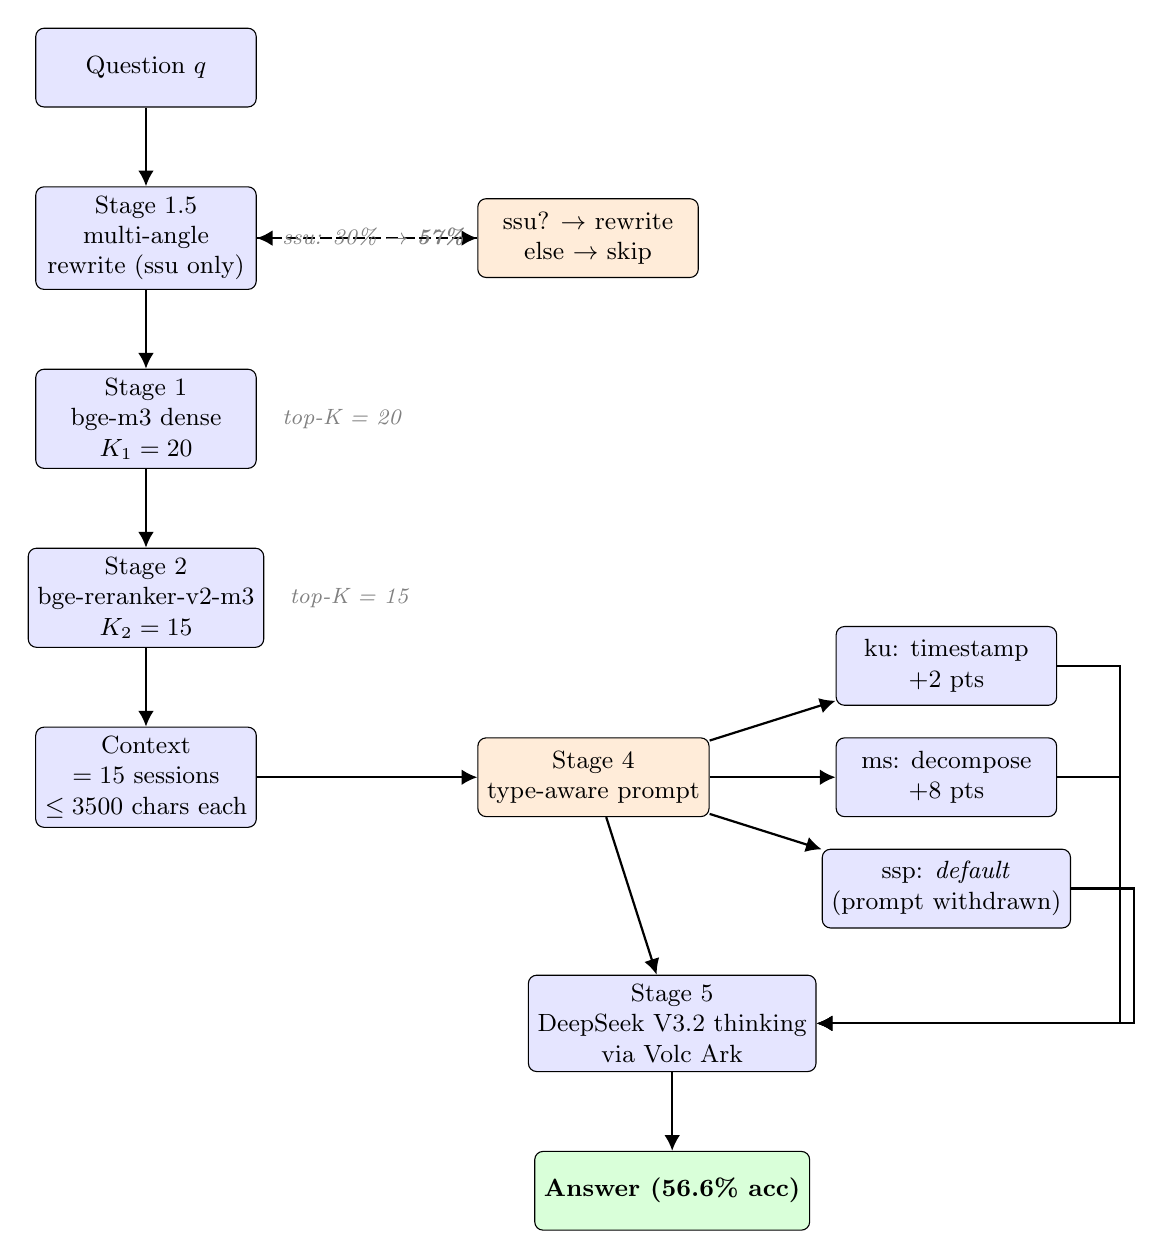
\begin{tikzpicture}[
    node distance=10mm and 8mm,
    box/.style={
      draw, rounded corners=3pt, minimum width=28mm, minimum height=10mm,
      align=center, font=\small
    },
    stage/.style={box, fill=blue!10},
    decision/.style={box, fill=orange!15},
    output/.style={box, fill=green!15, font=\small\bfseries},
    arrow/.style={-{Latex[length=2mm, width=2mm]}, thick},
    note/.style={font=\footnotesize\itshape, color=gray, align=center}
]

% Input
\node[stage] (q) {Question $q$};
\node[stage, below=of q] (qrw) {Stage 1.5\\multi-angle\\rewrite (ssu only)};
\node[stage, below=of qrw] (s1) {Stage 1\\bge-m3 dense\\$K_1=20$};
\node[stage, below=of s1] (s2) {Stage 2\\bge-reranker-v2-m3\\$K_2=15$};
\node[stage, below=of s2] (ctx) {Context\\$=15$ sessions\\$\le 3500$ chars each};

\node[decision, right=of qrw, xshift=20mm] (type) {ssu? $\to$ rewrite\\else $\to$ skip};

% Stage 4
\node[decision, right=of ctx, xshift=20mm] (s4) {Stage 4\\type-aware prompt};

\node[stage, right=of s4, xshift=8mm] (ms) {ms: decompose\\$+8$ pts};
\node[stage, above=4mm of ms] (ku) {ku: timestamp\\$+2$ pts};
\node[stage, below=4mm of ms] (ssp) {ssp: \emph{default}\\(prompt withdrawn)};

% LLM
\node[stage, below=20mm of s4, xshift=10mm] (llm) {Stage 5\\DeepSeek V3.2 thinking\\via Volc Ark};

% Output
\node[output, below=of llm] (ans) {Answer (56.6\% acc)};

% Arrows
\draw[arrow] (q) -- (qrw);
\draw[arrow] (qrw) -- (s1);
\draw[arrow] (s1) -- (s2);
\draw[arrow] (s2) -- (ctx);
\draw[arrow] (ctx) -- (s4);
\draw[arrow] (s4) -- (ms);
\draw[arrow] (s4) -- (ku);
\draw[arrow] (s4) -- (ssp);
\draw[arrow] (s4) -- (llm);
\draw[arrow] (ms.east) -- ++(8mm,0) |- (llm.east);
\draw[arrow] (ku.east) -- ++(8mm,0) |- (llm.east);
\draw[arrow] (ssp.east) -- ++(8mm,0) |- (llm.east);
\draw[arrow] (llm) -- (ans);

% Type decision feedback
\draw[arrow, dashed] (qrw) -- (type);
\draw[arrow, dashed] (type) -- (qrw);

% Notes
\node[note, right=2mm of qrw] {ssu: 30\% $\to$ \textbf{57\%}};
\node[note, right=2mm of s1] {top-K = 20};
\node[note, right=2mm of s2] {top-K = 15};

\end{tikzpicture}
\end{document}


\documentclass[border=8pt]{standalone}
\usepackage{tikz}
\usetikzlibrary{positioning, arrows.meta, shapes, fit, calc}

\begin{document}
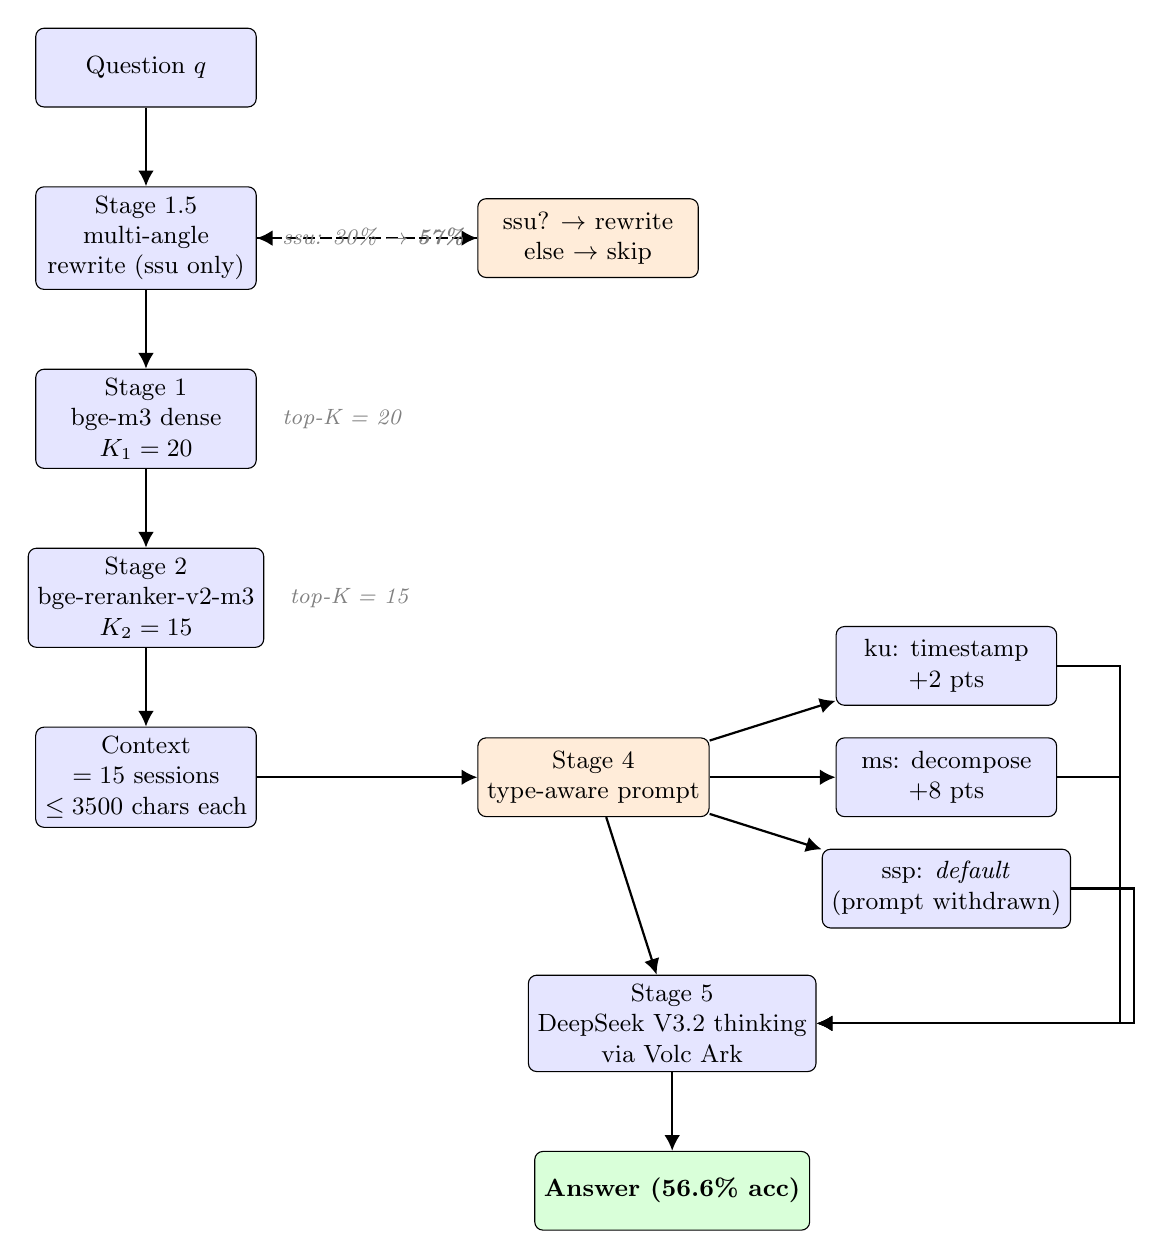
\begin{tikzpicture}[
    node distance=10mm and 8mm,
    box/.style={
      draw, rounded corners=3pt, minimum width=28mm, minimum height=10mm,
      align=center, font=\small
    },
    stage/.style={box, fill=blue!10},
    decision/.style={box, fill=orange!15},
    output/.style={box, fill=green!15, font=\small\bfseries},
    arrow/.style={-{Latex[length=2mm, width=2mm]}, thick},
    note/.style={font=\footnotesize\itshape, color=gray, align=center}
]

% Input
\node[stage] (q) {Question $q$};
\node[stage, below=of q] (qrw) {Stage 1.5\\multi-angle\\rewrite (ssu only)};
\node[stage, below=of qrw] (s1) {Stage 1\\bge-m3 dense\\$K_1=20$};
\node[stage, below=of s1] (s2) {Stage 2\\bge-reranker-v2-m3\\$K_2=15$};
\node[stage, below=of s2] (ctx) {Context\\$=15$ sessions\\$\le 3500$ chars each};

\node[decision, right=of qrw, xshift=20mm] (type) {ssu? $\to$ rewrite\\else $\to$ skip};

% Stage 4
\node[decision, right=of ctx, xshift=20mm] (s4) {Stage 4\\type-aware prompt};

\node[stage, right=of s4, xshift=8mm] (ms) {ms: decompose\\$+8$ pts};
\node[stage, above=4mm of ms] (ku) {ku: timestamp\\$+2$ pts};
\node[stage, below=4mm of ms] (ssp) {ssp: \emph{default}\\(prompt withdrawn)};

% LLM
\node[stage, below=20mm of s4, xshift=10mm] (llm) {Stage 5\\DeepSeek V3.2 thinking\\via Volc Ark};

% Output
\node[output, below=of llm] (ans) {Answer (56.6\% acc)};

% Arrows
\draw[arrow] (q) -- (qrw);
\draw[arrow] (qrw) -- (s1);
\draw[arrow] (s1) -- (s2);
\draw[arrow] (s2) -- (ctx);
\draw[arrow] (ctx) -- (s4);
\draw[arrow] (s4) -- (ms);
\draw[arrow] (s4) -- (ku);
\draw[arrow] (s4) -- (ssp);
\draw[arrow] (s4) -- (llm);
\draw[arrow] (ms.east) -- ++(8mm,0) |- (llm.east);
\draw[arrow] (ku.east) -- ++(8mm,0) |- (llm.east);
\draw[arrow] (ssp.east) -- ++(8mm,0) |- (llm.east);
\draw[arrow] (llm) -- (ans);

% Type decision feedback
\draw[arrow, dashed] (qrw) -- (type);
\draw[arrow, dashed] (type) -- (qrw);

% Notes
\node[note, right=2mm of qrw] {ssu: 30\% $\to$ \textbf{57\%}};
\node[note, right=2mm of s1] {top-K = 20};
\node[note, right=2mm of s2] {top-K = 15};

\end{tikzpicture}
\end{document}


\documentclass[border=8pt]{standalone}
\usepackage{tikz}
\usetikzlibrary{positioning, arrows.meta, shapes, fit, calc}

\begin{document}
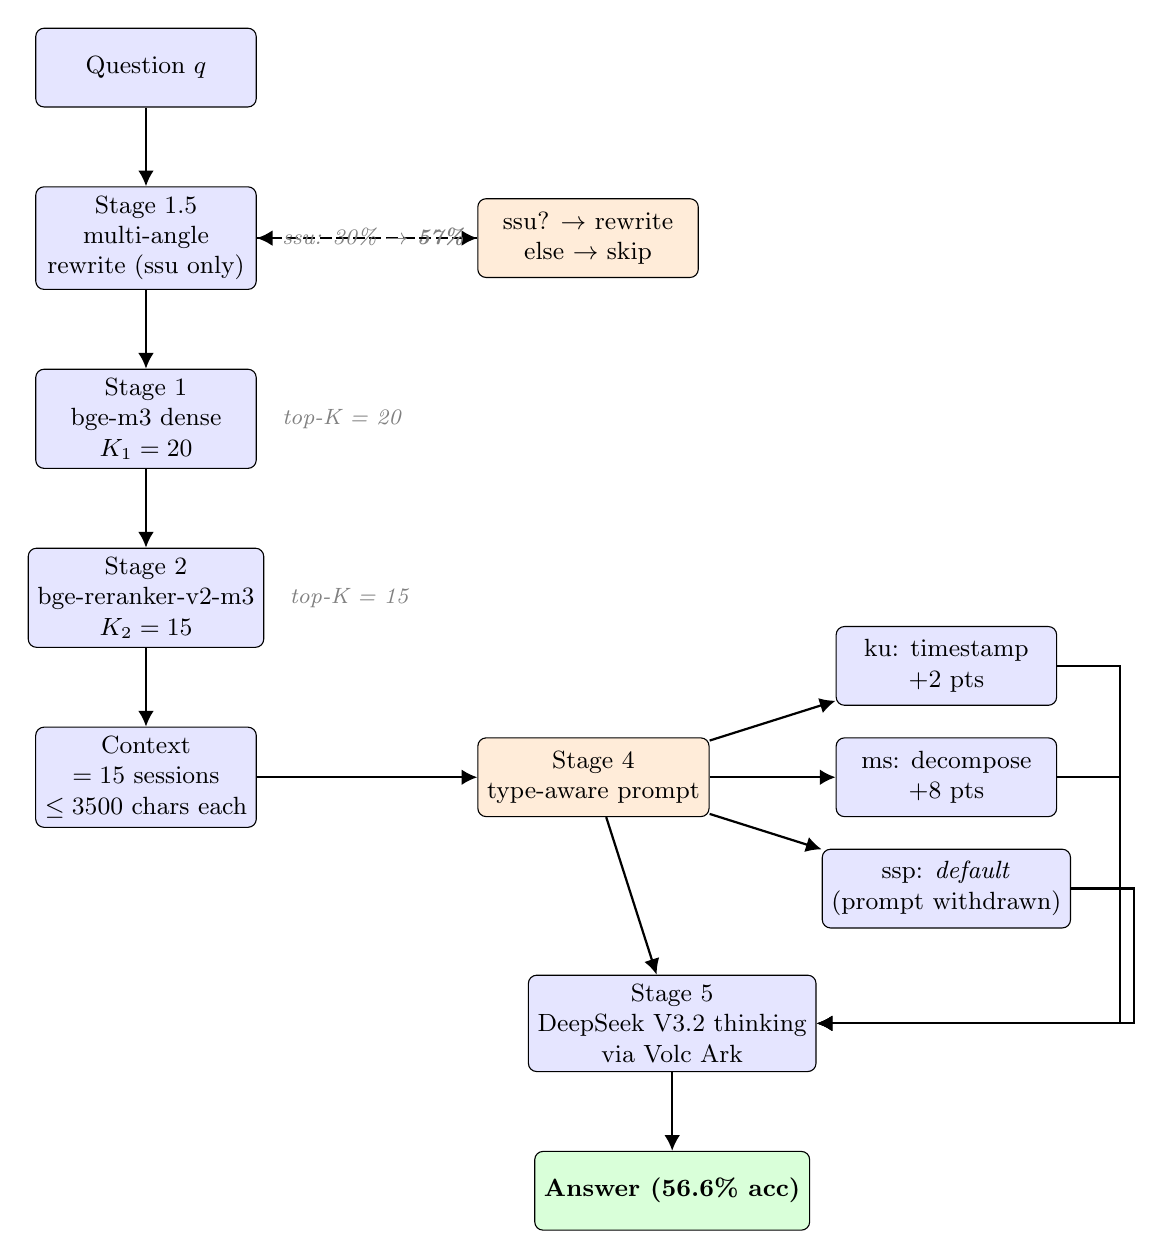
\begin{tikzpicture}[
    node distance=10mm and 8mm,
    box/.style={
      draw, rounded corners=3pt, minimum width=28mm, minimum height=10mm,
      align=center, font=\small
    },
    stage/.style={box, fill=blue!10},
    decision/.style={box, fill=orange!15},
    output/.style={box, fill=green!15, font=\small\bfseries},
    arrow/.style={-{Latex[length=2mm, width=2mm]}, thick},
    note/.style={font=\footnotesize\itshape, color=gray, align=center}
]

% Input
\node[stage] (q) {Question $q$};
\node[stage, below=of q] (qrw) {Stage 1.5\\multi-angle\\rewrite (ssu only)};
\node[stage, below=of qrw] (s1) {Stage 1\\bge-m3 dense\\$K_1=20$};
\node[stage, below=of s1] (s2) {Stage 2\\bge-reranker-v2-m3\\$K_2=15$};
\node[stage, below=of s2] (ctx) {Context\\$=15$ sessions\\$\le 3500$ chars each};

\node[decision, right=of qrw, xshift=20mm] (type) {ssu? $\to$ rewrite\\else $\to$ skip};

% Stage 4
\node[decision, right=of ctx, xshift=20mm] (s4) {Stage 4\\type-aware prompt};

\node[stage, right=of s4, xshift=8mm] (ms) {ms: decompose\\$+8$ pts};
\node[stage, above=4mm of ms] (ku) {ku: timestamp\\$+2$ pts};
\node[stage, below=4mm of ms] (ssp) {ssp: \emph{default}\\(prompt withdrawn)};

% LLM
\node[stage, below=20mm of s4, xshift=10mm] (llm) {Stage 5\\DeepSeek V3.2 thinking\\via Volc Ark};

% Output
\node[output, below=of llm] (ans) {Answer (56.6\% acc)};

% Arrows
\draw[arrow] (q) -- (qrw);
\draw[arrow] (qrw) -- (s1);
\draw[arrow] (s1) -- (s2);
\draw[arrow] (s2) -- (ctx);
\draw[arrow] (ctx) -- (s4);
\draw[arrow] (s4) -- (ms);
\draw[arrow] (s4) -- (ku);
\draw[arrow] (s4) -- (ssp);
\draw[arrow] (s4) -- (llm);
\draw[arrow] (ms.east) -- ++(8mm,0) |- (llm.east);
\draw[arrow] (ku.east) -- ++(8mm,0) |- (llm.east);
\draw[arrow] (ssp.east) -- ++(8mm,0) |- (llm.east);
\draw[arrow] (llm) -- (ans);

% Type decision feedback
\draw[arrow, dashed] (qrw) -- (type);
\draw[arrow, dashed] (type) -- (qrw);

% Notes
\node[note, right=2mm of qrw] {ssu: 30\% $\to$ \textbf{57\%}};
\node[note, right=2mm of s1] {top-K = 20};
\node[note, right=2mm of s2] {top-K = 15};

\end{tikzpicture}
\end{document}


\documentclass[border=8pt]{standalone}
\usepackage{tikz}
\usetikzlibrary{positioning, arrows.meta, shapes, fit, calc}

\begin{document}
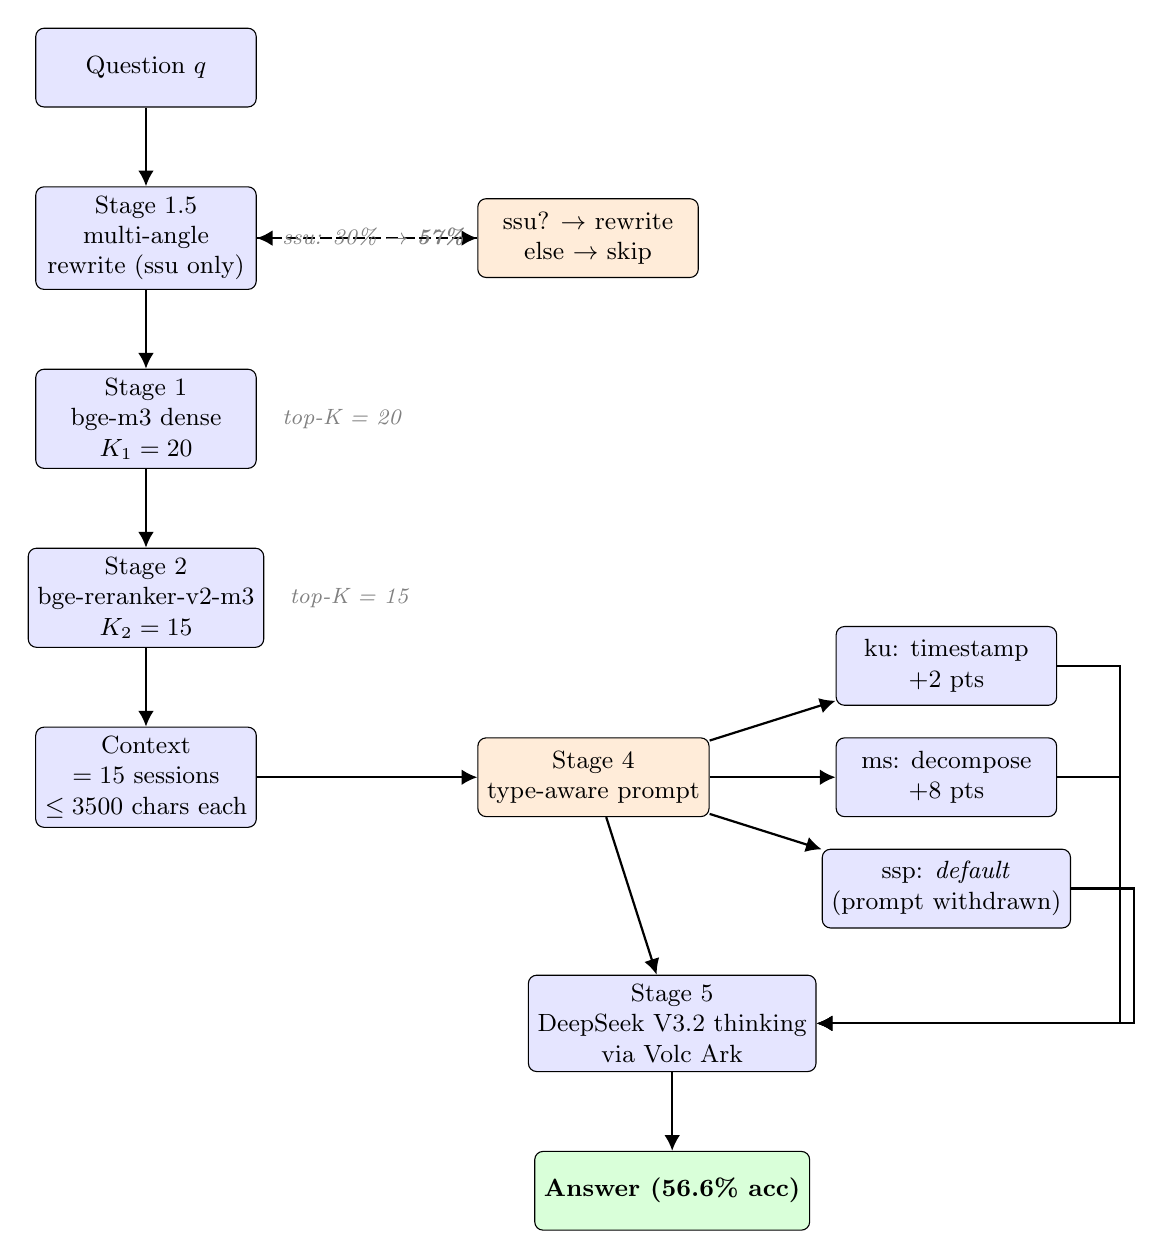
\begin{tikzpicture}[
    node distance=10mm and 8mm,
    box/.style={
      draw, rounded corners=3pt, minimum width=28mm, minimum height=10mm,
      align=center, font=\small
    },
    stage/.style={box, fill=blue!10},
    decision/.style={box, fill=orange!15},
    output/.style={box, fill=green!15, font=\small\bfseries},
    arrow/.style={-{Latex[length=2mm, width=2mm]}, thick},
    note/.style={font=\footnotesize\itshape, color=gray, align=center}
]

% Input
\node[stage] (q) {Question $q$};
\node[stage, below=of q] (qrw) {Stage 1.5\\multi-angle\\rewrite (ssu only)};
\node[stage, below=of qrw] (s1) {Stage 1\\bge-m3 dense\\$K_1=20$};
\node[stage, below=of s1] (s2) {Stage 2\\bge-reranker-v2-m3\\$K_2=15$};
\node[stage, below=of s2] (ctx) {Context\\$=15$ sessions\\$\le 3500$ chars each};

\node[decision, right=of qrw, xshift=20mm] (type) {ssu? $\to$ rewrite\\else $\to$ skip};

% Stage 4
\node[decision, right=of ctx, xshift=20mm] (s4) {Stage 4\\type-aware prompt};

\node[stage, right=of s4, xshift=8mm] (ms) {ms: decompose\\$+8$ pts};
\node[stage, above=4mm of ms] (ku) {ku: timestamp\\$+2$ pts};
\node[stage, below=4mm of ms] (ssp) {ssp: \emph{default}\\(prompt withdrawn)};

% LLM
\node[stage, below=20mm of s4, xshift=10mm] (llm) {Stage 5\\DeepSeek V3.2 thinking\\via Volc Ark};

% Output
\node[output, below=of llm] (ans) {Answer (56.6\% acc)};

% Arrows
\draw[arrow] (q) -- (qrw);
\draw[arrow] (qrw) -- (s1);
\draw[arrow] (s1) -- (s2);
\draw[arrow] (s2) -- (ctx);
\draw[arrow] (ctx) -- (s4);
\draw[arrow] (s4) -- (ms);
\draw[arrow] (s4) -- (ku);
\draw[arrow] (s4) -- (ssp);
\draw[arrow] (s4) -- (llm);
\draw[arrow] (ms.east) -- ++(8mm,0) |- (llm.east);
\draw[arrow] (ku.east) -- ++(8mm,0) |- (llm.east);
\draw[arrow] (ssp.east) -- ++(8mm,0) |- (llm.east);
\draw[arrow] (llm) -- (ans);

% Type decision feedback
\draw[arrow, dashed] (qrw) -- (type);
\draw[arrow, dashed] (type) -- (qrw);

% Notes
\node[note, right=2mm of qrw] {ssu: 30\% $\to$ \textbf{57\%}};
\node[note, right=2mm of s1] {top-K = 20};
\node[note, right=2mm of s2] {top-K = 15};

\end{tikzpicture}
\end{document}
